\chapter{Wstęp}
\label{ch:wstep}

\section{Cel pracy}
Przedmiotem niniejszej pracy jest przegląd metod rozwiązujacych zagadnienie planowania bezkolizyjnych tras dla wielu robotów. Stanowi to również wstęp teoretyczny do zaprojektowania algorytmu i implementacji oprogramowania pozwalającego na symulację działania systemu planowania tras.

Praca skupia się na przypadkach, w których mamy do czynienia ze środowiskiem z dużą liczbą przeszkód (np. zamknięty budynek z licznymi ciasnymi korytarzami), gdzie problem blokowania sią agentów prowadzi często do zakleszczenia. Należy wtedy zastosować nieco inne podejścia niż te, które sprawdzają się w przypadku otwartych środowisk, a które zostały opisane np. w pracach: \cite{roszkowska}, \cite{siemiatkowska}

W niniejszej pracy zajmować będziemy się rozwiązaniem problemu, w którym mamy pełną informację o mapie otoczenia oraz o określonym położeniu początkowym i celu dla każdego z robotów. Zadaniem algorytmu będzie wyznaczenie możliwie najkrótszej bezkolizyjnej trasy dla wszystkich robotów. Należy jednak zaznaczyć, że priorytetem jest dotarcie każdego z robotów do celu bez kolizji z innymi robotami, dopiero później chcemy, aby wyznaczone drogi były możliwie najkrótsze.

\section{Koordynacja ruchu robotów}
Koordynacja ruchu robotów jest jednym z fundamentalnych problemów w systemach wielu robotów. \cite{optpriorities}

Kooperacyjne znajdowanie tras (ang. Cooperative Pathfinding) jest problemem planowania w układzie wieloagentowym, w którym to agenci mają za zadanie znaleźć bezkolizyjne drogi do swoich, osobnych celów. Planowanie to odbywa się w oparciu o pełną informację o środowisku oraz trasach pozostałych agentów. \cite{cooppath}

Problem kooperacyjnego znajdowania tras pojawia się często m.in. w grach komputerowych, gdzie należy wyznaczyć drogi dla wielu jednostek, które mogą blokować się wzajemnie. Algorytmy do wyznaczania bezkolizyjnych tras dla wielu agentów (robotów) mogą znaleźć również zastosowanie w szpitalach (np. roboty TUG i HOMER do dostarczania sprzętu na wyposażeniu szpitala \cite{tughomer}) oraz magazynach (np. roboty transportowe w magazynach firmy Amazon \cite{amazonrobots}).

\section{Przestrzeń konfiguracyjna}
Przestrzeń konfiguracyjna to formalna, matematyczna przestrzeń będąca zbiorem możliwych stanów danego układu fizycznego.
W zależności od rodzaju i liczby wyróżnionych parametrów stanu przestrzenie konfiguracyjne mogą mieć wiele wymiarów.

\section{Metoda hill-climbing}
Metoda hill-climbing jest rodzajem matematycznej optymalizacji, lokalną metodą przeszukiwania.
Jest to iteracyjny algorytm, który zaczyna w wybranym rozwiązaniu problemu, następnie próbuje znaleźć lepsze rozwiązanie poprzez przyrostowe zmiany pojedynczych elementów rozwiązania.
Jeśli zmiana przynosi lepsze rozwiązanie, jest wprowadzana do nowego rozwiązania.
Kroki algorytmu powtarzane są dotąd, aż żadne ``udoskonalenie'' nie zostaje znalezione.

\chapter{Metody planowania tras}
\label{ch:path_planning_methods}

\section{Metody planowania tras}
Spośród metod wykorzystywanych do planowania tras dla wielu robotów można wyróżnić dwie zasadnicze grupy \cite{latombe}:
\begin{itemize}
	\item {\bf Zcentralizowane} - drogi wyznaczane są dla wszystkich agentów na raz (jednocześnie). Metody te potrafią znaleźć wszystkie możliwe rozwiązania (w szczególności to optymalne), ale mają bardzo dużą złożoność obliczeniową ze względu na ogromną przestrzeń przeszukiwania. Z tego powodu stosowane są heurystyki przyspieszające proces obliczania rozwiązania.
	\item {\bf Rozproszone} (ang. {\it decoupled} lub {\it distributed}) - Podejście to dekomponuje zadanie na niezależne lub zależne w niewielkim stopniu problemy dla każdego agenta. Dla każdego robota droga wyznaczana jest osobno, w określonej kolejności, następnie rozwiązywane są konflikty (kolizje dróg). W pewnych przypadkach rozwiązanie może nie zostać znalezione, mimo, iż istnieje. Zastosowanie metod rozproszonych wiąże się najczęściej z koniecznością przydzielenia priorytetów robotom, co stanowi istotny problem, gdyż od ich wyboru może zależeć zupełność algorytmu. Nie należy mylić tej metody z zagadnieniem typu {\it Non-Cooperative Pathfinding}, w którym agenci nie mają wiedzy na temat pozostałych planów i muszą przewidywać przyszłe ruchy pozostałych robotów \cite{cooppath}. W podejściu rozproszonym agenci mają pełną informację na temat stanu pozostałych robotów, lecz wyznaczanie dróg odbywa się w określonej kolejności.
\end{itemize}

\subsection{Metody zcentralizowane}
Wiele metod zcentralizowanych cechuje się planowaniem w zbiorowej przestrzeni konfiguracyjnej oraz możliwością wyznaczenia optymalnego rozwiązania.
Wadą jest natomiast duża złożoność obliczeniowa algorytmu i konieczność posiadania pełnej informacji o stanie otoczenia i robotów.

W systemach czasu rzeczywistego istotne jest, aby rozwiązanie problemu planowania tras uzyskać w określonym czasie, dlatego w tego typu sytemach częściej używane są techniki rozproszone.

\subsection{Metoda sztucznych pól potencjałowych}
Nie wszystkie podejścia zcentralizowane gwarantują optymalne rozwiązanie. Przykładem takiej metody, która nie daje gwarancji optymalności (ani nawet zupełności) jest metoda sztucznych pól potencjałowych.

Metoda sztucznych pól potencjałowych (ang. {\it Artificial Potential Field}) polega na zastosowaniu zasad oddziaływania między ładunkami znanych z elektrostatyki. Roboty i przeszkody traktowane są jako ładunki jednoimienne, przez co "odpychają się" siłą odwrotnie proporcjonalną do kwadratu odległości (dzięki temu unikają kolizji). Natomiast punkt docelowy robota jest odwzorowany jako ładunek o przeciwnym biegunie, przez co robot jest "przyciągany" do celu.
Główną zasadę działania metody przedstawiono na rysunku \ref{fig:image_potentialfield}.
Technika jest bardzo prosta i nie wymaga wykonywania złożonych obliczeń (w odróżnieniu do pozostałych metod zcentralizowanych). Niestety bardzo powszechny jest problem osiągania minimum lokalnego, w którym suma wektorów daje zerową siłę wypadkową. Robot zostaje "uwięziony" w minimum lokalnym, przez co nie jest w stanie dotrzeć do wyznaczonego celu. Do omijania tego problemu muszą być stosowane inne dodatkowe metody. \cite{potentialfield}
\begin{figure}[H]
	\centering
	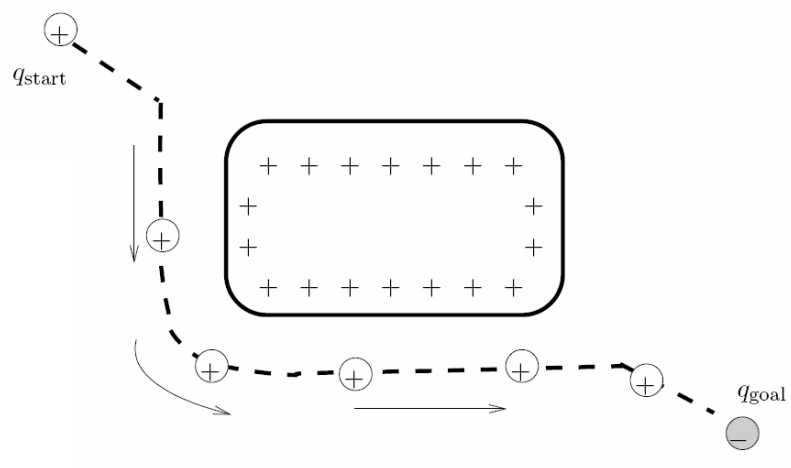
\includegraphics[width=12cm]{img/potential-field}
	\caption{Zasada działania metody sztucznych pól potencjałowych. Źródło: \cite{howie_potentialfield}}
	\label{fig:image_potentialfield}
\end{figure}

\subsection{Rozproszone wyznaczanie tras}
Popularne podejścia unikające planowania w wysoko wymiarowej zbiorowej przestrzeni konfiguracyjnej to techniki rozproszone i priorytetowane.
Pomimo, że metody te są bardzo efektywne, mają dwie główne wady:
\begin{enumerate}
	\item Nie są zupełne - czasami nie udaje się znaleźć rozwiązania, nawet gdy istnieje.
	\item Wynikowe rozwiązania są często nieoptymalne.
\end{enumerate}

W artykule \cite{optpriorities} przedstawione zostało podejście do optymalizowania układu priorytetów dla rozproszonych i priorytetowanych technik planowania.
Proponowana metoda wykonuje randomizowane przeszukiwanie z techniką hill-climbing do znalezienia rozwiązania i do skrócenia całkowitej długości ścieżek.
Technika ta została zaimplemenotwana i przetestowana na prawdziwych robotach oraz w rozległych testach symulacyjnych.
Wyniki eksperyentu pokazały, że metoda potrafi znacząco zmniejszyć liczbę niepowodzeń i znacznie zmniejszyć całkowitą długość tras dla różnych priorytetowanych i rozproszoncyh metod planowania dróg, nawet dla dużych zespołów robotów.

Najczęściej stosowanymi podejściami są metody oparte o algorytm A*. W szczególności są to:
\begin{itemize}
	\item A* w konfiguracji czaso-przestrzennej
	\item Path coordination
\end{itemize}

\subsubsection{Path coordination}
Idea metody Path coordination przedstawia się następująco \cite{optpriorities}:
\begin{enumerate}
	\item Wyznaczenie ścieżki dla każdego robota {\bf niezależnie}
	\item Przydział priorytetów
	\item Próba rozwiązania możliwych konfliktów między ścieżkami. Roboty utrzymywane są na ich indywidualnych ścieżkach (wyznaczonych na początku), wprowadzane modyfikacje pozwalają na zatrzymanie się, ruch naprzód, a nawet cofanie się, ale tylko {\bf wzdłuż trajektorii} w celu uniknięcia kolizji z robotem o wyższym priorytecie.
\end{enumerate}
Złożoność metody wynosi $O(n \cdot m \cdot log(m))$, $m$ - maksymalna liczba stanów podczas planowania, $n$ - liczba robotów

\subsection{Wybór priorytetów}
$TODO$ nie dotyczy tylko Path coordination, ale też A* time-space
Istotną rolę doboru priorytetów robotów w procesie planowania tras ukazuje prosty przykład przedstawiony na rysunku \ref{fig:image_article1_fig1}. Jeśli robot 1 (zmierzający z punktu S1 do G1) otrzyma wyższy priorytet niż robot 2 (zmierzający z S2 do G2), spowoduje to zablokowanie przejazdu dla robota 2 i w efekcie prawidłowe rozwiązanie nie zostanie znalezione.
\begin{figure}[H]
	\centering
	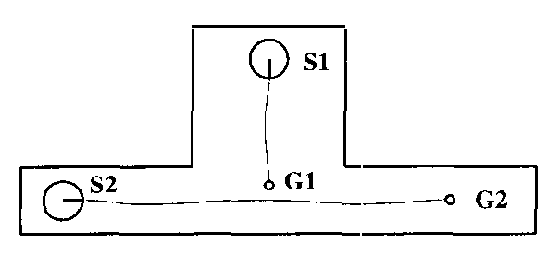
\includegraphics[width=10cm]{img/article1/fig1}
	\caption{Sytuacja, w której żadne rozwiązanie nie zostanie znalezione, jeśli robot 1 ma wyższy priorytet niż robot 2. Źródło: \cite{optpriorities}}
	\label{fig:image_article1_fig1}
\end{figure}

Układ priorytetów może mieć również zasadniczy wpływ na długość uzyskanych tras. Odpowiedni przykład został przedstawiony na rysunku \ref{fig:image_article1_ppt6}. W zależności od wyboru priorytetów, wpływających na kolejność planowania tras, otrzymujemy różne rozwiązania.
\begin{figure}[H]
	\centering
	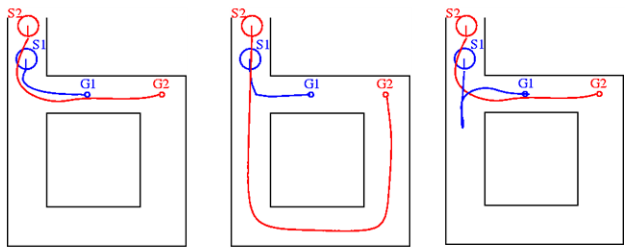
\includegraphics[width=13cm]{img/article1/ppt6}
	\caption{a) Niezależne planowanie optymalnych tras dla 2 robotów; b) suboptymalne rozwiązanie, gdy robot 1 ma wyższy priorytet; c) rozwiązanie, gdy robot 2 ma wyższy priorytet}
	\label{fig:image_article1_ppt6}
\end{figure}
